\makeatletter
   \def\input@path{{.}}
\makeatother

\documentclass[
    % colors = false,
    geometry = 16k,
]{LALUbook}

\usepackage{mathdots}
\usepackage{booktabs} % Excel 导出的大表格
\usepackage{rotating}
\usepackage{extarrows}

\usepackage{float}
\usepackage{diagbox}
\usepackage{caption}

\usepackage{pgfplots}
\usetikzlibrary{cd, arrows, arrows.meta, calc, intersections, decorations.pathreplacing, patterns, decorations.markings,angles,quotes}
\pgfplotsset{compat=newest}

\usepackage[xindy, splitindex]{imakeidx}
\makeindex[
    columns=1,
    program=truexindy,
    intoc=true,
    options=-M texindy -I xelatex -C utf8,
    title={名词索引}
] % 名词索引
\makeindex[
    columns=3,
    program=truexindy,
    intoc=true,
    options=-M numeric-sort -M latex -M latex-loc-fmts -M makeindex -I xelatex -C utf8,
    name=sym,
    title={符号索引}
] % 符号索引

% 嵌套 enumerate 环境的 label
\setlist[enumerate,2]{label=(\arabic*)}
\setlist[enumerate,3]{label=\roman*.}

\usepackage{xparse}
\NewDocumentCommand{\term}{m}{{\sffamily\heiti\bfseries{#1}}}

\newcounter{LUchapter}
\newcounter{LUgreekchap}

\makeatletter
% 此处可按需增改
% \texorpdfstring 的两个参数分别显示在正文中与 PDF 书签中
\newcommand*{\@LUgreek}[1]{%
    \ifcase#1\or\texorpdfstring{$\boldsymbol{\varepsilon}$}{ε}%
    \or\texorpdfstring{$\boldsymbol{\delta}$}{δ}%
    \or\texorpdfstring{$\boldsymbol{\lambda}$}{λ}%
    \or\texorpdfstring{$\boldsymbol{\mu}$}{μ}%
    \or\texorpdfstring{$\boldsymbol{\varphi}$}{φ}%
    \or\texorpdfstring{$\boldsymbol{\theta}$}{θ}%
    \else\@ctrerr\fi%
}
\newcommand*{\LUgreek}[1]{%
    \expandafter\@LUgreek\csname c@#1\endcsname
}
\newcommand*{\LUchapsancheck}{%
\expandafter\@ifundefined{@exist@LUchapter@\arabic{chapter}.\arabic{LUgreekchap}}%
    {\setcounter{LUgreekchap}{1}}
    {\stepcounter{LUgreekchap}}
}
\newcommand*{\LUgroupsancheck}{%
\expandafter\@ifundefined{@exist@LUchapter@\arabic{chapter}}%
    {}
    {\endgroup}
}

\let\@std@chapter\chapter
\renewcommand*{\chapter}{%
    \LUgroupsancheck%
    \@std@chapter
}
\makeatother

% 内容总结
\newenvironment{summary}{%
    \hypersetup{bookmarksnumbered=false}%
    \titleformat{\subsection}[block]{\centering\Large}{}{1em}{}%
    \subsection{内容总结}%
}{}

% 习题环境
% \begin{exercise}
%   \exquote[somebody]{...}
%   \begin{exgroup}
%     \item ...
%     \item ...
%   \end{exgroup}
%   \begin{exgroup}
%     ...
%   \end{exgroup}
% \end{exercise}
\newcounter{exgroupcounter}
\newenvironment{exercise}{%
    \setcounter{exgroupcounter}{0}%
    \NewDocumentEnvironment{exgroup}{so}{%
        \IfBooleanF{##1}{%
            \IfValueTF{##2}{%
                \setcounter{exgroupcounter}{##2}%
            }{%
                \refstepcounter{exgroupcounter}%
            }%
            \subsection{\Alph{exgroupcounter} 组}%
        }%
        \begin{enumerate}%
    }{%
        \end{enumerate}%
    }%
    \NewDocumentCommand{\exquote}{om}{%
        \vspace{2ex}%
        {\sffamily\kaishu ##2}%
        \IfValueT{##1}{%
            \begin{flushright}%
                \sffamily\kaishu ——##1%
            \end{flushright}%
        }%
    }%
    \hypersetup{bookmarksnumbered=false}%
    \titleformat{\section}[block]{\centering\Large}{}{1em}{}%
    \titleformat{\subsection}[block]{\centering\bfseries}{}{1em}{}%
    \section{习题}%
}{}

\NewDocumentCommand{\LUchapter}{m}{%
\LUgroupsancheck
\begingroup
\LUchapsancheck
\addtocounter{chapter}{-1}
\refstepcounter{LUchapter}
\renewcommand*{\thechapter}{\arabic{chapter}\LUgreek{LUgreekchap}}
\renewcommand*{\theHchapter}{LU.\arabic{LUchapter}}
\ctexset{
    chapter={format={\centering\Huge\bfseries},name={未竟专题,},number={\zhnumber{\arabic{LUchapter}}}},
}
\csname @std@chapter\endcsname{#1}
\expandafter\xdef\csname @exist@LUchapter@\arabic{chapter}\endcsname{\relax}
\expandafter\xdef\csname @exist@LUchapter@\arabic{chapter}.\arabic{LUgreekchap}\endcsname{\relax}
}

\ctexset{
    chapter={format={\centering\Huge\bfseries},name={第,讲},number=\arabic{chapter}},
    section={format={\raggedright\Large\bfseries},name={,},number={\thechapter.\arabic{section}}},
    subsection={format={\raggedright\large\bfseries},name={,},number={\thesection.\arabic{subsection}}},
    subsubsection={format={\raggedright\normalsize\bfseries},name={,},number={\thesubsection.\arabic{subsubsection}}},
}

\title{Probability and Statistics for Information Science Lecture Notes}
\author{Hengyu Ai}
\date{Fall 2024}

\AtEndPreamble{\hypersetup{
    hypertexnames=true,
    pdfauthor={Hengyu Ai},
    pdftitle={SI140A Notes},
}}

\begin{document}
\frontmatter

\maketitle

\songti

\pagenumbering{Roman}

\pdfbookmark[0]{目录}{contents}
\tableofcontents

\addtolength{\parskip}{.5em}

\mainmatter
% 定义
% \begin{definition}{标题}{引用标签}\index{glossary用的拼音@glossary 内容}
% content
% \end{definition}

% 定理
% \begin{theorem}{标题}{引用标签} 
% content
% \end{theorem}

% \begin{equation}\label{eq:2:引用标签}
%   content
% \end{equation}

% 引用定义
% \autoref{def:引用标签}

% 引用定理
% \autoref{thm:引用标签}

% 引用等式
% \autoref{eq:2:引用标签}

% 同理,引理 -> lemma lem
%       例子 -> example ex
%       推论 -> corollary cor

\chapter{概率与计数 Probability and Counting}

\section{概率模型 Probabilistic Model}

\begin{definition}{集合}{集合}\index{jihe@集合 (Set)}
    
    \begin{enumerate}
        \item 空集: $\emptyset$
        \item 子集(subset)关系:$A \subseteq B$
        \item 交(union):$A \cup B$
        \item 并(intersection):$A \cap B$
        \item 补(complement):$A^c$
        \item De Morgan 律:$(A \cup B)^c = A^c \cap B^c, (A \cap B)^c = A^c \cup B^c$
    \end{enumerate}
    
\end{definition}

\begin{definition}{样本空间(Sample Space)}{样本空间}
    一个实验的全部可能的结果的集合称为\term{样本空间}.
\end{definition}

\begin{definition}{事件(event)}{事件}
    样本空间的子集称为\term{事件}.
    
    当实际结果属于一个事件时,称这个事件发生 (occured)
\end{definition}


\begin{tabular}{ll}
    \toprule
    \textbf{English} & \textbf{Sets} \\
    \midrule
    \textit{Events and occurrences} & \\
    sample space & \(S\) \\
    \(s\) is a possible outcome & \(s \in S\) \\
    \(A\) is an event & \(A \subseteq S\) \\
    \(A\) occurred & \(s_{\text{actual}} \in A\) \\
    something must happen & \(s_{\text{actual}} \in S\) \\
    \midrule
    \textit{New events from old events} & \\
    \(A\) or \(B\) (inclusive) & \(A \cup B\) \\
    \(A\) and \(B\) & \(A \cap B\) \\
    not \(A\) & \(A^c\) \\
    \(A\) or \(B\), but not both & \((A \cap B^c) \cup (A^c \cap B)\) \\
    at least one of \(A_1, \ldots, A_n\) & \(A_1 \cup \cdots \cup A_n\) \\
    all of \(A_1, \ldots, A_n\) & \(A_1 \cap \cdots \cap A_n\) \\
    \midrule
    \textit{Relationships between events} & \\
    \(A\) implies \(B\) & \(A \subseteq B\) \\
    \(A\) and \(B\) are mutually exclusive & \(A \cap B = \emptyset\) \\
    \(A_1, \ldots, A_n\) are a partition of \(S\) & \(A_1 \cup \cdots \cup A_n = S, \, A_i \cap A_j = \emptyset \text{ for } i \neq j\) \\
    \bottomrule
\end{tabular}

\newpage

\section{概率与计数的朴素定义}

\subsection{概率}

\begin{definition}{概率(朴素定义)}{概率naive}
    假设:
    \begin{enumerate}
        \item 有限样本空间
        \item 输出结果等可能
    \end{enumerate}
    
    则:
    
    令 $A$ 为一个事件,$S$ 为其样本空间,则 $A$ 的概率为
    
    $$
    P_{naive}(A) = \frac{|A|}{|P|} = \frac{\text{number of outcomes favorable to } A}{\text{total number of outcomes in } S}
    $$
    
    在这种情况下概率被转化为计数问题。
\end{definition}

\begin{example}{Pascal-Fermat Correspondence}{PF Bet Game}
    Alice 和 Bob 抛硬币,三次获胜的人赢。每一轮 Alice 赌注硬币为正面 (Head),Bob 赌注反面 (Tail)。当前比分为 $2 : 1$,若此时结束游戏该如何按可能的结果划分奖品?\\
    
    在第五轮游戏必然结束,则剩下两局样本空间为:$S = \{HH, HT, TH, TT\}$,当且仅当投出 $TT$ 时 Bob 获胜,则应该给 Alice $\dfrac{3}{4}$,给 Bob $\dfrac{1}{4}$
\end{example}

\subsection{计数}

\begin{itemize}
    \item \textbf{Sampling}: 从集合等可能获取一个元素
    \item \textbf{With Replacement \& without replacement}: 取出后放回/不放回
    \item \textbf{Ordered \& Unorderd}
\end{itemize}

\begin{example}{生日问题}{生日问题}
    房间内有 $k$ 人,假设一个人生日为一年 $365$ 天内等可能随机一天,生日互相独立,求至少两人有相同生日的概率。\\
    
    相当于从集合 $\{1, 2, 3, \dots, 365\}$ 取出 $k$ 个元素,with replacement。令 $A$ 表示“存在两人以上……“的情况,则 $A^c$ 为”没有任何人和别人生日相同“的情况。\\
    
    $$
    P(A^c) = \frac{|A^c|}{|S|} = \frac{\text{without replacement 的 samples}}{\text{with replacement}} = \frac{365!}{365^k} (k \leqslant 365)
    $$
    
    $$
    P(A) = 1 - P(A^c)
    $$
    
\end{example}

\begin{theorem}{广义生日问题}{GBirthday}
    从 $n$ 个值中随机选 $k$ 次,当 $k \approx 1.18 \sqrt{n}$ 时,有 50\% 的概率,至少有两个选取的值相同。\\
    
    考虑按每个随机变量来计算 $P(A^c)$, 则第一个变量从 $[1, n]$ 选择任意,第二变量必须取到和第一个不同的,第三个取和一、二不同的,并且变量之间相互独立,以此类推:
    
    $$
    P(A^c) = \frac{n}{n} \times \frac{n - 1}{n} \times \frac{n - 2}{n} \cdots \times \frac{n - (k - 1)}{n} = \prod_{i = 1}^{k} \frac{n - i}{n}
    $$
    
    当 $n \gg k$ 时,$\dfrac{n - i}{n} = 1 - \dfrac{i}{n} \approx \mathrm{e}^{-\frac{i}{n}}$,于是 $\prod \frac{n - i}{n} = \mathrm{e}^{-\frac{1 + 2 + \cdots + k - 1}{n}} = \mathrm{e}^{-\frac{k (k - 1)}{2n}} \approx \mathrm{e}^{-\frac{k^2}{2n}}$
    
    于是 $P(A) \approx 1 - \mathrm{e}^{-\frac{k^2}{2n}}$
    
    代入 $P(A) = 0.5$ 得出 $k = \sqrt{n \cdot 2 \ln 2} \approx 1.18 \sqrt{n}$
    
\end{theorem}

\begin{theorem}{多项式定理(Multinomial Theorem)}{Multinomial Theorem}
    $$
    (x_1 + x_2 + x_3 + \dots + x_r)^n = \sum_{n_1, n_2, \dots, n_r \geqslant 0} \frac{n!}{n_1 ! n_2 ! \cdots n_r !} x_1^{n_1} x_2^{n_2} \cdots x_r^{n_r} (n_1 + n_2 + \cdots + n_r = n)
    $$
    
    组合意义:把 $n$ 个不同的人分成 $r$ 组
\end{theorem}

在证明组合恒等式时,可以使用式子两侧组合意义说明等式成立。

\begin{theorem}{吸收/提取恒等式}{AEIdentity}
    $$
    n \binom{n - 1}{k - 1} = k \binom{n}{k}
    $$
\end{theorem}

\begin{proof}
    假设有如下场景:从 $n$ 人中选出 $k$ 个组成小队,并且这 $k$ 人中有一人为小队长。\\
    
    \autoref{thm:AEIdentity} LHS 可以视为先选出小队长($n$ 种方案),然后在剩下的 $n - 1$ 人中选出小队剩余成员(组合数). RHS 可以视为先从 $n$ 人中选出组成小队的 $k$ 人(组合数),然后在小队内部选出队长($k$ 种方案),可知等式成立。
\end{proof}

\begin{theorem}{Vandermonde 卷积}{Vandermonde}
    
    $$
    \binom{m + n}{k} = \sum_{j = 0}^{k} \binom{m}{j} \binom{n}{k - j}
    $$
    
\end{theorem}

\begin{proof}
    假设有如下场景:有 $m$ 个男生和 $n$ 个女生,从中选出 $k$ 个人作为一组。\\
    
    \autoref{thm:Vandermonde} LHS 即为直接选择,RHS 为,枚举从男生中选出几个人($j$ 从 $0$ 到 $k$),然后选出 $\binom{m}{j}$ ,再从女生中选出剩下的人($\binom{n}{k - j}$)
\end{proof}

\begin{theorem}{Bose-Einstein 计数定理}{BECounting}
    组合意义:可重复选择,顺序无影响,从 $n$ 中选 $k$\\
    
    形式描述:$x_1 + x_2 + \cdots + x_n = k, x_i \in \mathbb{N}, i = 0, 1, 2, \dots, n$, 这个不定方程的解的个数为
    
    $$
    \binom{n + k - 1}{n - 1}
    $$
    
    类似的,当解要求必须为正时,可以按照\textbf{隔板法}求解
\end{theorem}

\begin{example}{}{}
    求如下方程解的个数:
    
    $$
    x_1 + x_2 + x_3 + x_4 = 88, x_1 \ge 3, x_2 \ge 5, x_3 \ge 8, x_4 \ge 10
    $$
    
    令 $y_1 = x_1 - 3, y_2 = x_2 - 5, y_3 = x_3 - 8, y_4 = x_4 - 10$,转化为 \autoref{thm:BECounting}
    
\end{example}

选择 \( n \) 个对象中的 \( k \) 个对象,可能的方式数量:

\begin{center}

\begin{tabular}{|c|c|c|}
\hline
& 顺序有关 & 顺序无关 \\
\hline
允许放回 & \( n^k \) & \( \displaystyle \binom{n+k-1}{k} \) \\
\hline
不允许放回 & \( n(n-1) \cdots (n-k+1) \) & \( \displaystyle \binom{n}{k} \) \\
\hline
\end{tabular}

\end{center}

\section{其他非公理化的概率定义}

\subsection{无限样本空间中的概率}

按照测度理论的几何度量定义。

\begin{example}{}{}
    随机变量 $x \in [0, 3]$, 求 $x$ 到 $0$ 比到 $1$ 更近的概率.\\
    
    一维的几何度量为线段长度:
    
    $$
    P(A) = \frac{\text{Length of } [0, 0.5]}{\text{Length of } [0, 3]}
    $$
\end{example}

\begin{example}{}{}
    随机变量 $x \in [1, 2]$, 求 $P(x = 1.5)$\\
    
    将 $[1, 2]$ 分为 $[1, 1 + \frac{1}{2n + 1}), [1 + \frac{1}{2n + 1}, 1 + \frac{2}{2n + 1}), \cdots$
    
    可知对任何一个区间, $P(x \in [l, r)) = \dfrac{1}{2n + 1}$
    
    $$
    \forall n \ge 1, 0 \ge P(x = 1.5) \le P(x \in A_n) = \dfrac{1}{2n + 1}
    $$
    
    令 $n \to \infty$, 可知 $P(x = 1.5) = 0$
\end{example}

在上面的例子中,出现了概率为 $0$ 的事件,但是那个事件并不是不可能时间。

一个不可能事件概率为 $0$,概率为 $0$ 的事件为\textbf{事件测度为 0},不代表事件不会发生。

更高维度也有相似的测度定义的概率:

\begin{example}{}{}
    在一个正方形中均匀任取一点,求这个点在正方形内接圆的概率。
    \begin{center}
    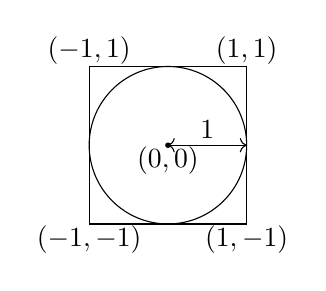
\begin{tikzpicture}

    % Draw the square
    \draw (-1, -1) rectangle (1, 1);
    
    % Draw the circle
    \draw (0, 0) circle (1);
    
    % Draw the arrow
    \draw[->] (0,0) -- (1,0);
    \draw[<-] (0,0) -- (1,0);
    \node at (0.5, 0.2) {1};
    
    % Draw points
    \fill (0,0) circle (1pt);
    
    % Add coordinates
    \node at (-1, 1.2) {$(-1,1)$};
    \node at (1, 1.2) {$(1,1)$};
    \node at (-1, -1.2) {$(-1,-1)$};
    \node at (1, -1.2) {$(1,-1)$};
    \node at (0, -0.2) {$(0,0)$};
    
    \end{tikzpicture}
    \end{center}
    
    二维的测度使用面积衡量。
    
    $$
    P(A) = \frac{S_{\text{circle}}}{S_{\text{square}}} = \frac{\pi}{4}
    $$
    
\end{example}

\subsection{统计定义的概率}

概率是重复一个实验很多次后得到的频率。

\textbf{大数定理,Monte Carlo 方法}

\newpage

\section{公理化的概率定义}

\begin{definition}{公理化的概率}{概率}
    给定样本空间 $S$,构成事件类的 $S$ 子集满足如下公理
    
    \begin{enumerate}
        \item $S$ 是一个事件
        \item 对于任何事件 $A$,其补集是事件
        \item 可列的数个事件的并是事件
    \end{enumerate}
    
    概率函数 $P: A \to \mathbb{R}$ 满足如下公理
    
    \begin{enumerate}
        \item $P(\emptyset) = 0, P(S) = 1$
        \item 对于互不相交的事件 $A_1, A_2, \dots$
    \end{enumerate}
    
    $$
    P\left(\bigcup_{j = 1}^{\infty} A_j \right) = \sum_{j = 1}^{\infty} P(A_j)
    $$
\end{definition}

根据上述概率的公理,可以导出一些概率的性质:

\begin{itemize}
    \item $P(A^c) = 1 - P(A)$
    \item 若 $A \subseteq B$,则 $P(A) \leq P(B)$
    \item $P(A \cup B) = P(A) + P(B) - P(A \cap B)$
\end{itemize}

\begin{theorem}{容斥原理}{IEFormula}
    对于任何 $n$ 个事件 $A_1, A_2, \dots, A_n$
    
    $$
    P\left(\bigcup_{i = 1}^{n} A_i\right) = \sum_i P(A_i) - \sum_{i < j} P(A_i \cap A_j) + \cdots + (-1)^{n + 1} P(A_1 \cap A_2 \cap \cdots \cap A_n)
    $$
\end{theorem}

\begin{example}{De Montmort 匹配问题}{}
    从均匀洗牌的 $n$ 张卡的卡堆内,卡按照 $1 \sim n$ 标号,逐张翻开卡牌,若有任何一次满足翻开第 $k$ 张时,那张牌标号为 $k$ 则获胜。
    
    令 $A_i$ 表示第 $i$ 张开的牌标号为 $i$ 的事件,则 $P(\text{win}) = P(A_1 \cap A_2 \cap \cdots \cap A_n)$
    
    $P(A_i) = \dfrac{1}{n}$
    
    根据对称性,$P(A_i \cup A_j \cup A_k \cdots \cup A_p)$ 对于相同的 $p$ 都相同
    
    $$
    P(A_i \cup A_j \cup A_k \cdots \cup A_p) = 
    $$
\end{example}

用于分析具有不确定结果的现象的框架:
\begin{itemize}
    \item 保持一致推理的规则
    \item 用于预测和决策
\end{itemize}

\begin{center}

\begin{tikzpicture}[node distance=3cm]
    \node [square, draw] (realworld) {现实世界};
    \node [square, draw] (inference) [below of=realworld] {推理/统计};
    \node [square, draw] (probability) [right of=inference, xshift=2cm] {概率论(分析)};

    \draw [->] (realworld) -- node[anchor=east] {数据} (inference);
    \draw [->] (inference) -- node[anchor=south] {模型} (probability);
    \draw [->] (probability) -- node[anchor=west] {预测/决策} (realworld);

\end{tikzpicture}

\end{center}

\input{./src/Lecture02.tex}
\input{./src/Lecture03.tex}
% 定义
% \begin{definition}{标题}{引用标签}\index{glossary用的拼音@glossary 内容}
% content
% \end{definition}

% 定理
% \begin{theorem}{标题}{引用标签} 
% content
% \end{theorem}

% \begin{equation}\label{eq:2:引用标签}
%   content
% \end{equation}

% 引用定义
% \autoref{def:引用标签}

% 引用定理
% \autoref{thm:引用标签}

% 引用等式
% \autoref{eq:2:引用标签}

% 同理,引理 -> lemma lem
%       例子 -> example ex
%       推论 -> corollary cor

\chapter{期望}

\begin{summary}



\end{summary}

\input{./src/Lecture05.tex}
\input{./src/Lecture06.tex}
\input{./src/Lecture07.tex}
\input{./src/Lecture08.tex}
\input{./src/Lecture09.tex}
\input{./src/Lecture10.tex}

\LUgroupsancheck

\makeatletter
\let\chapter\@std@chapter
\let\@std@chapter\relax
\makeatother

\backmatter
{\small
\printindex
\printindex[sym]
}

\end{document}
